% ============================================================
%  Chapter 7 — Conclusion
% ============================================================
\chapter{Conclusion}
\label{ch:conclusion}

\section{Summary}

This report presented an intrinsic image decomposition model trained with
Cross-Render Albedo Invariance (CARI).
The central problem we addressed is the leakage of coloured illumination into the
predicted albedo: when a room is lit by a warm yellow lamp, standard IID models
tend to predict a slightly yellow version of the wall's true colour because they
have no mechanism to distinguish the lamp's hue from the material's hue.

CARI attacks this problem at the training stage rather than the model stage.
By presenting the model with pairs of images of the same scene photographed under
different coloured lights, and penalising any change in the predicted albedo
between the two images, we force the model to assign all the illuminant colour
information to the shading layer.
This approach requires two practical ingredients: a dataset with real multi-illuminant
pairs (we use MID), and a commitment to not applying white balance to those pairs.
White balance neutralises the illuminant colour before training, which removes the
very signal that CARI needs to operate.

Establishing this required repairing the instrument before we could trust the reading.
The chroma-cast score we had inherited and used in earlier drafts of this work
pools albedo chromaticity across all the materials of a scene before taking its variance,
and so measures the scene's ordinary chromatic diversity alongside the illuminant-induced
drift it is intended to isolate. That diversity term is computed from the model's own
prediction, which makes the score reducible by a model that simply desaturates its albedo.
The metric, in other words, paid models to destroy the quantity intrinsic decomposition
exists to recover. It ranked the configuration of our own model whose albedo is visibly
drained of colour as the best in the ablation, and the colour-preserving configuration as
the worst. Decomposing the score into a scale-normalised invariance term and a calibration
term anchored on MID pseudo-ground truth reverses that verdict and brings the
numbers back into agreement with what the images plainly show
(\secref{sec:mid_results}, \figref{fig:chroma_fidelity}).

Our experiments then compare CARI against a matched no-CARI baseline and against
external methods across four benchmarks: MID and ARAP for colour-illuminant
constancy, MAW for measured albedo accuracy, and IIW for perceptual shading
quality (\chapref{ch:experiments}).
The result is a conjunction rather than a clean sweep, and we state it as such. Our model
is the only one in the comparison that is simultaneously colour-faithful and competitively
invariant: it closely matches the MID pseudo-GT chroma calibration and
holds the best material-lightness stability in the roster. It does \emph{not} hold the
best hue-invariance score; two external methods do. The fidelity guard shows why
that ranking is not the compliment it appears to be: both of them buy their invariance by
discarding real albedo colour, one of them to very nearly the same degree as the ablated
configuration of our own model that we discarded on sight. Where we trail on IIW, the
evidence only establishes weaker sparse relative-reflectance ordering. More decisively,
fine-tuning directly for IIW lowers WHDR by $17\%$ while worsening MID lightness constancy by
$47\%$, MAW colour error by $30\%$, and MAW intensity error by $69\%$. The benchmark gain
therefore hides damage to the constancy and measured-albedo properties central to this thesis.

The ablation identifies the reliable causal result: real cross-illuminant pairs
improve constancy when the colour path is held fixed. The later refinement study
is deliberately weaker evidence because its rows do not all share an identical
data mixture; it records useful trade-offs without claiming that every change is
caused by one isolated factor.


\section{Limitations}

Our approach has several limitations that future work could address.
\figref{fig:limitations} shows two measured failure modes directly, because most other qualitative
figure in this thesis shows the method working and that is not, on its own, evidence of
anything.

\begin{figure}[t!]
  \centering
  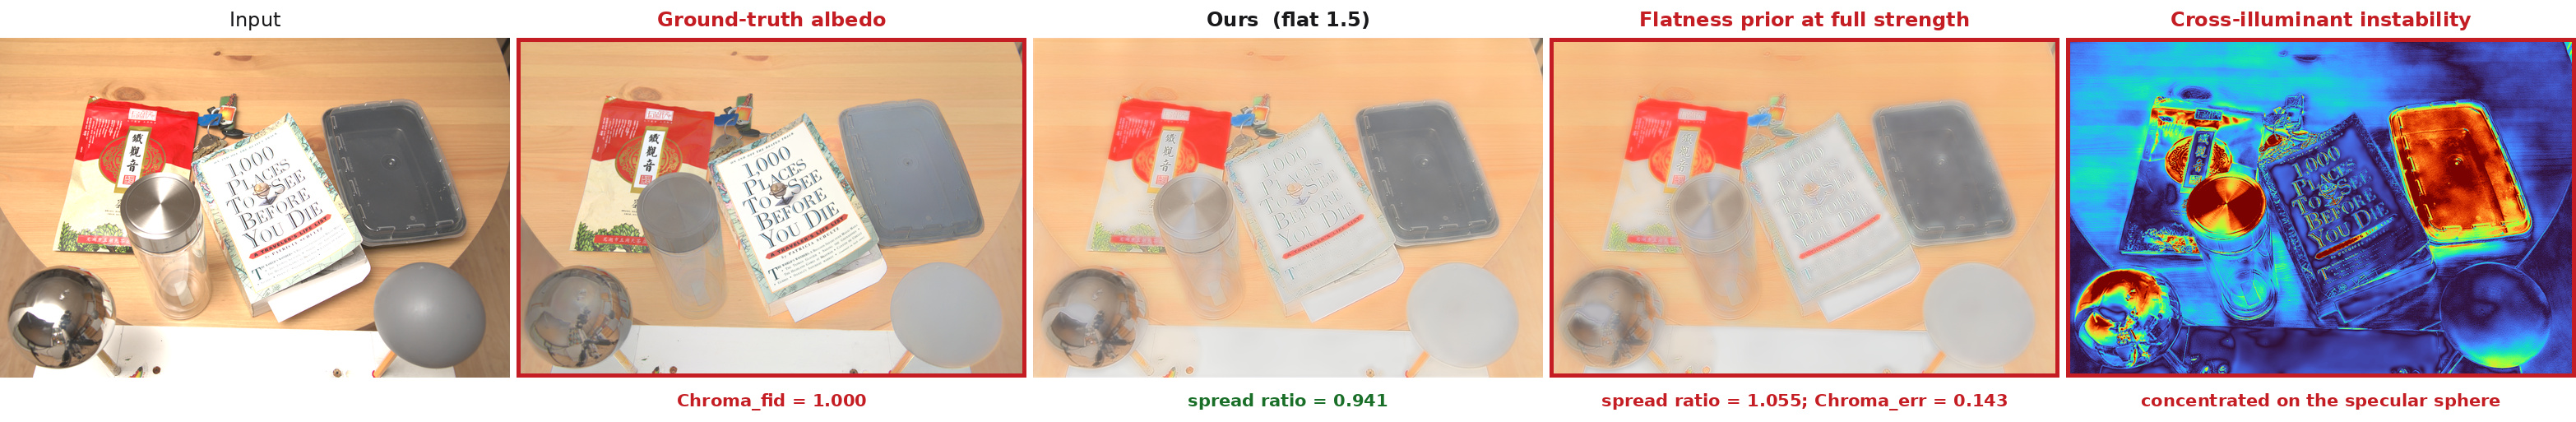
\includegraphics[width=\textwidth]{images/limitations/limitations.jpg}
  \caption[Representative limitations: flatness and non-diffuse surfaces.]{%
    Where the method fails. From left: the input; the ground-truth albedo; our selected
    model; the same model with the flatness prior at full strength; and a per-pixel map of
    how much our predicted albedo moves when only the illuminant moves.
    \textbf{The flatness prior is not free.} At full strength (Table-B Row~5) it does not
    merely smooth texture. It is associated with an aggregate chroma-spread ratio of
    $1.055$, compared with $0.941$ for the selected model, and costs a quarter of a
    $\Delta E$ unit on MAW. Because the recorded data mixtures differ, this does not
    isolate the flatness weight causally; it documents the failure of the full Row~5
    configuration.
    \textbf{Non-diffuse surfaces remain unsolved.} The instability map is not uniform: it
    concentrates on the mirrored sphere and the glossy lid. An albedo--shading product has
    no representation for a mirror, so the residual absorbs what it can and the rest
    surfaces as cross-illuminant drift.
  }
  \label{fig:limitations}
\end{figure}

\paragraph{Constancy-structure trade-off}
As described in \secref{sec:iiw_results}, the model does not simultaneously
achieve its best constancy and its best WHDR.
The fine-tuning diagnostic shows that the two objectives can pull in opposite directions:
improving sparse relative-reflectance ordering damages both material-lightness stability and
measured albedo accuracy.
Resolving this tension likely requires an explicit model of the illuminant,
so the network can separate material colour from illuminant colour more cleanly
rather than just being constrained not to let them mix.

\paragraph{Invariance cannot be optimised for on its own}
The metric correction of \secref{sec:mid_results} is not merely a bookkeeping fix; it
constrains what any future work on this problem may claim. A perfectly constant predictor
(one that emits flat grey albedo regardless of its input) is \emph{perfectly}
illuminant-invariant, and will score better on any pure drift measure than any model that
actually recovers colour. Invariance is therefore not a quantity that can be reported, or
optimised, in isolation: it is only meaningful paired with a fidelity term that is
anchored on an external albedo reference rather than on the model's own output. MID
provides a dataset-derived pseudo-reference; MAW supplies the independently measured
check. We suspect this
degeneracy is not peculiar to our formulation, since the pooled score we inherited exhibits
it, and we note that two of the four external methods we evaluate lead the uncorrected
score while measurably discarding albedo colour. A systematic audit of how colour constancy
is scored elsewhere in the IID literature is beyond the scope of this thesis, but our
result suggests it would be worth conducting.

\paragraph{Achromatic ambiguity}
Even with perfect coloured-illuminant constancy, a different fundamental ambiguity
remains: a dark textured surface (say, a dark grey carpet with visible pile) can
look similar to a lighter surface under a slight shadow.
This achromatic texture-shading confusion is not resolved by CARI, which only
deals with coloured differences between images.
It is the fundamental ill-posedness of IID, and addressing it requires geometric
priors or cross-image consistency beyond what CARI provides.

\paragraph{Scale of multi-illuminant training data}
MID contains approximately 1,000 scenes, but it is still much smaller and less
varied than the synthetic corpora used for supervised IID training.
The constancy constraint is therefore applied to a relatively limited set of
scene-illuminant combinations, which limits how much the model can generalise.
More multi-illuminant data, especially with a wider variety of illuminant colours
and surface materials, would likely improve the constancy further.

\paragraph{Grey shading assumption in the loss, not the representation}
The model's shading output is three-channel (\secref{sec:physics}), so it can
represent spatially varying illuminant colour in principle.
What remains grey-biased in practice is the \emph{supervision}: the
ground-truth shading available from Hypersim is achromatic, so the
three-channel shading head is disambiguated toward colour almost entirely by
CARI on MID pairs, which is a comparatively small and less spatially diverse
signal.
A scene with two differently coloured light sources active in different
regions of the same image is not well represented in either training source,
which limits how finely the model can localise a spatially mixed illuminant.


\section{Future Work}

Several directions follow naturally from this work.

\paragraph{Stronger and more plentiful invariance signals}
The ablation points toward the signal itself: more cross-illuminant pairs,
covering more materials and a wider range of illuminant colours, would directly
strengthen the constraint that does the work in our approach.
A structured illuminant representation (for example, a small palette of
illuminant colours with a spatial assignment map) remains an interesting
direction for representing \emph{spatially mixed} illuminants, but our
current evidence suggests it should be pursued as a complement to a strong
invariance signal, not as a substitute for one.

\paragraph{Quantifying the enhancement application}
\chapref{ch:practice} demonstrates that the recovered decomposition supports
qualitative edits (residual suppression and factor-space illumination adjustment)
without any additional training.
A natural extension is to evaluate these edits quantitatively, for example by
user studies on perceived realism of edited images, or downstream enhancement
metrics, thereby turning the qualitative demonstration into
a measured application.

\paragraph{Evaluation on additional coloured-illuminant benchmarks}
The Beigpour MIID dataset \mycite{beigpour13miid} (\secref{sec:multiillum})
provides real scenes with multiple coloured light sources and ground-truth
illuminant annotations.
If access becomes available, evaluating on it would test the model on a more controlled version of the
multi-illuminant problem and provide a comparison point with multi-illuminant
colour-constancy methods, in addition to the IID methods compared in
\chapref{ch:experiments}.
